\section{Description of the System}
The project I have chosen is called \textbf{FridgeIO}. It is a web application designed to help users keep track of the food they have at home and monitor expiration dates directly from the web browser. The main purpose of the system is to provide an accessible overview of household food supplies, thereby reducing food waste and supporting better meal planning.

\begin{figure}[!h]
    \centering
    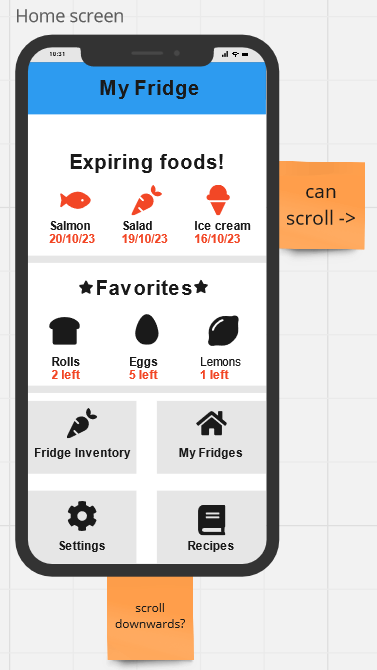
\includegraphics[width=0.5\linewidth]{images/HomescreenWireframe.png}
    \caption{Wireframe of FridgeIO}
    \label{fig:Wireframe}
\end{figure}

As illustrated in the wireframe in Figure~\ref{fig:Wireframe}, the central goal of FridgeIO is to give users an intuitive overview of their household inventory. The application is designed as a mobile-first solution, allowing users to quickly check their stock while in the store or standing in front of the fridge. This design focus emphasizes ease of use in everyday scenarios.

In addition to inventory management, FridgeIO supports recipe creation within the application. Recipes are intended to automatically remove the required ingredients from the user's “fridge” when the recipe is prepared, thereby streamlining the process of cooking with available ingredients.

The prototype was hosted on NTNU's SkyHigh server and used a NoSQL cloud database for flexible data storage. The frontend was implemented in React with ViteJS, and communication with the database was managed through a REST API. The project was developed collaboratively in a group of four students, integrating knowledge from multiple courses into one product.

\begin{figure}[!ht]
    \centering
    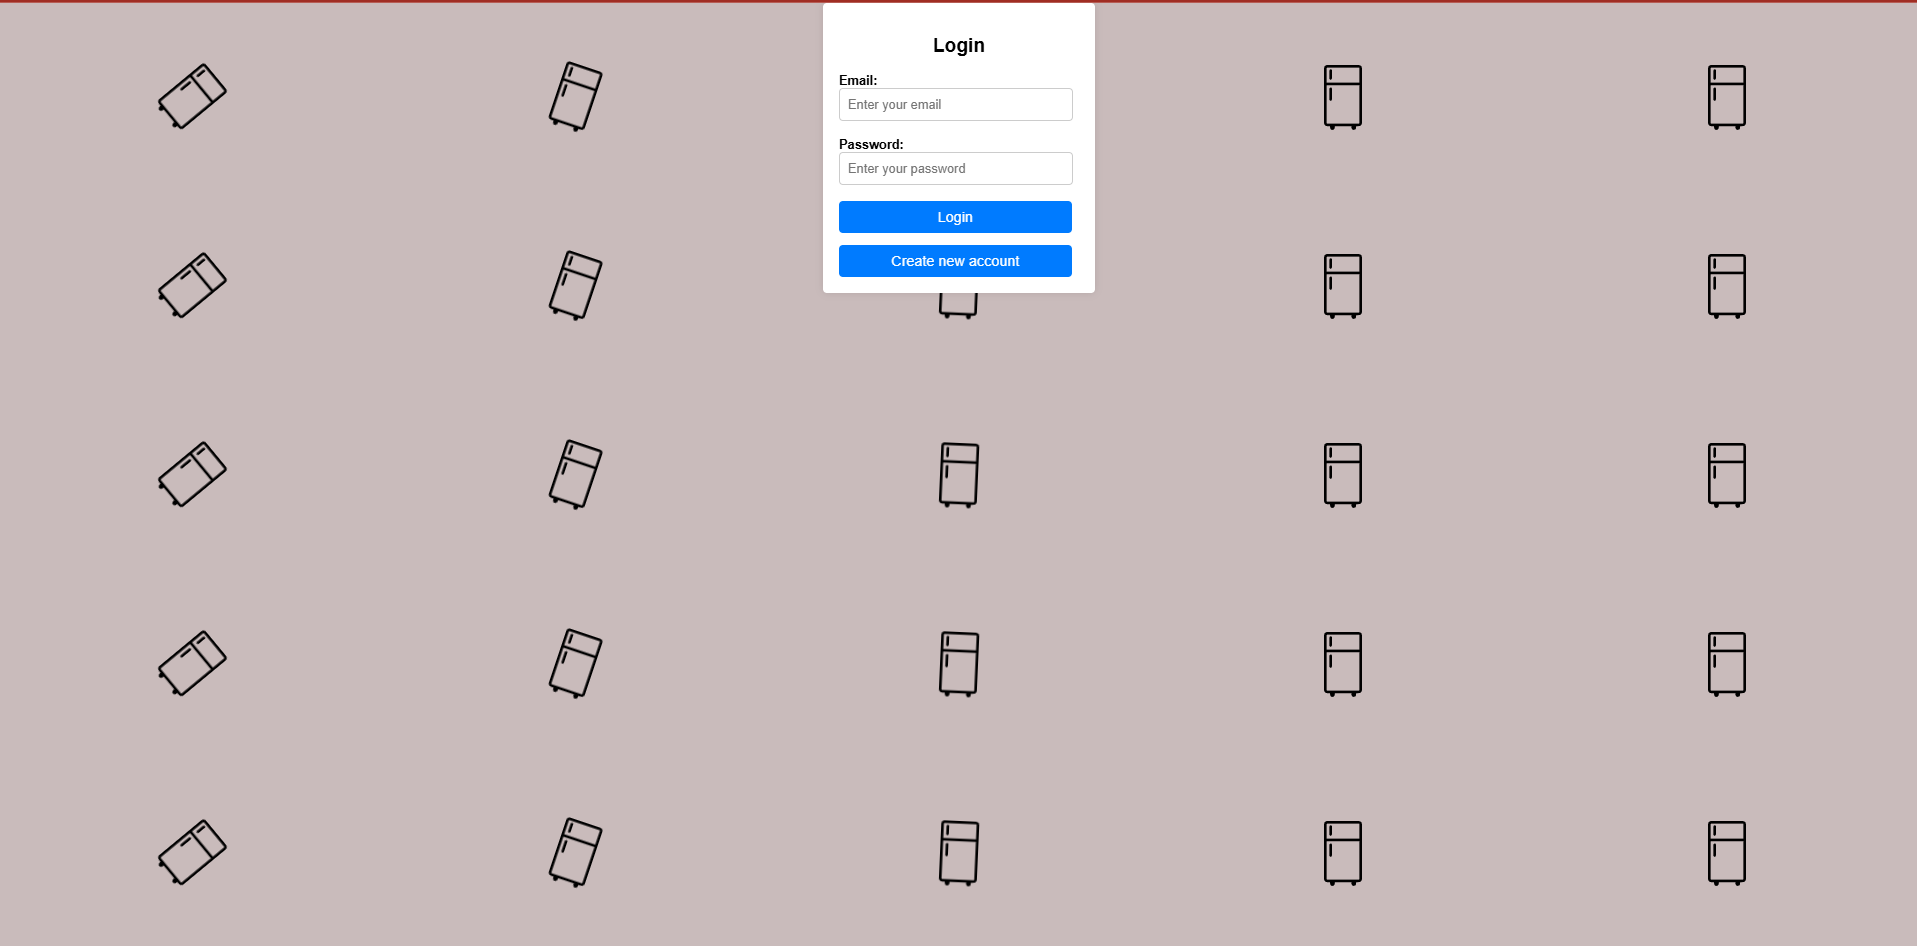
\includegraphics[width=0.8\linewidth]{images/FridgeIOLogin.png}
    \caption{FridgeIO Login Page}
    \label{fig:FridgeIOLogin}
\end{figure}

\begin{figure}[!ht]
    \centering
    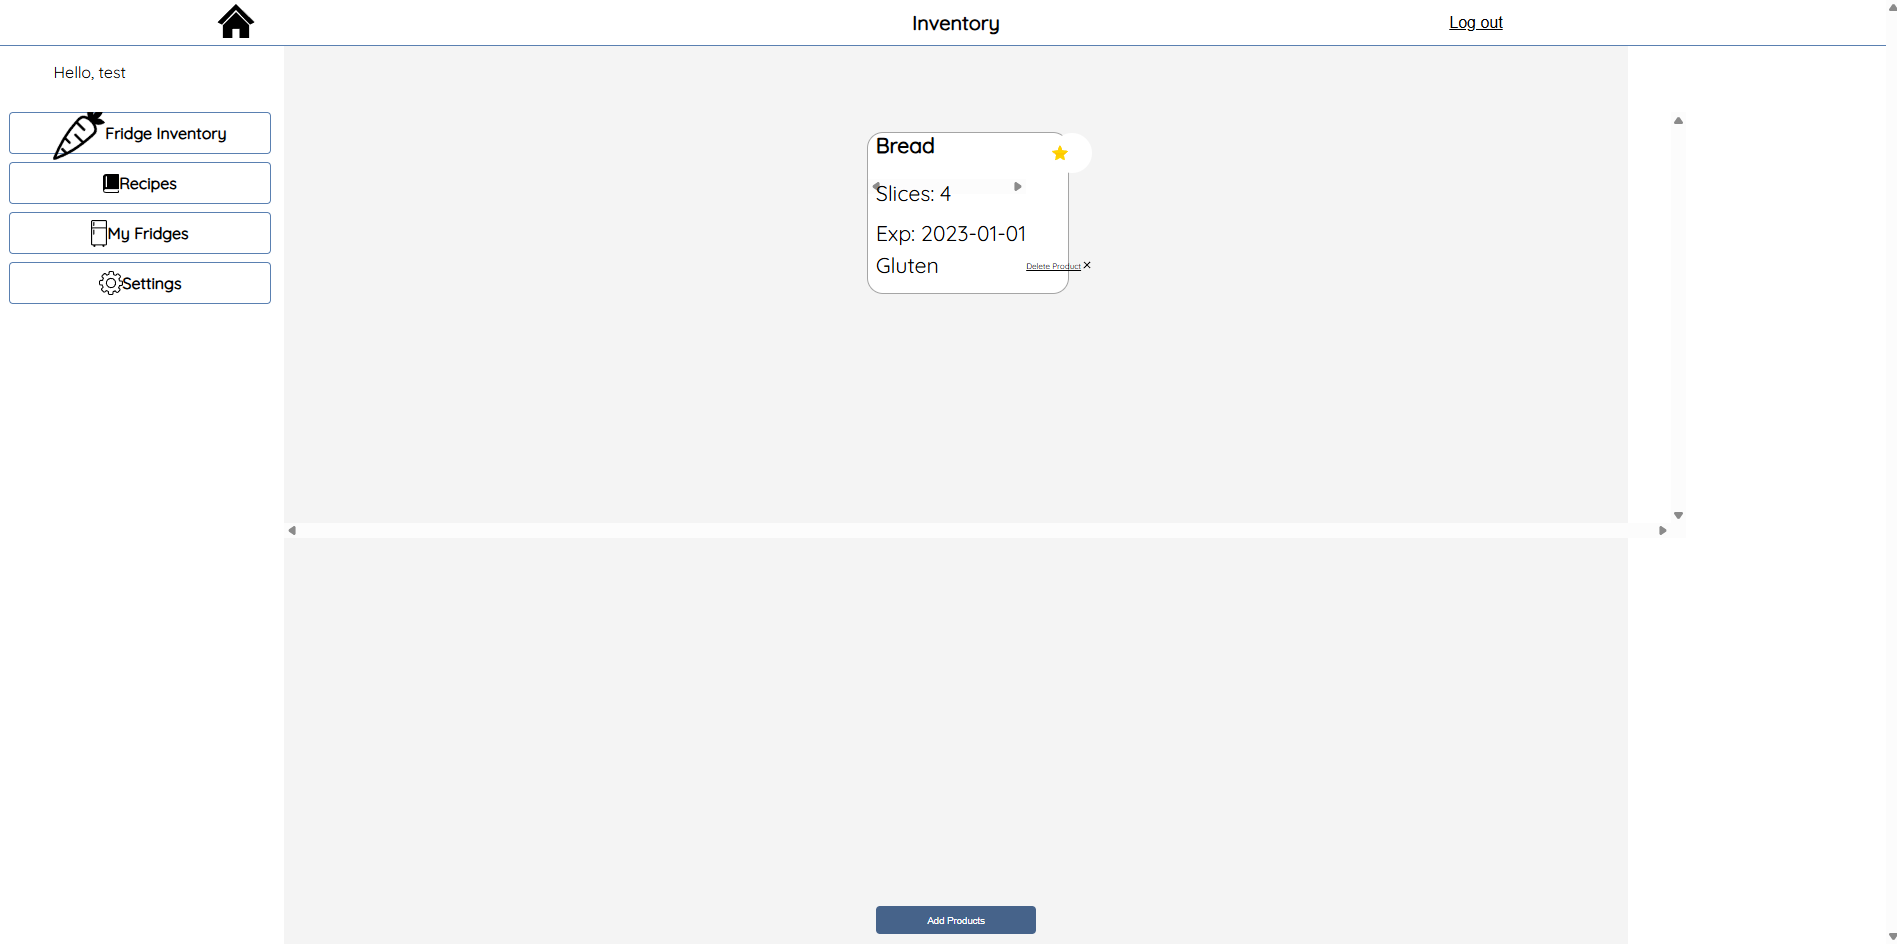
\includegraphics[width=0.8\linewidth]{images/fridgeIO.png}
    \caption{FridgeIO Main Page}
    \label{fig:FridgeIOMain}
\end{figure}

As seen in Figures~\ref{fig:FridgeIOLogin} and \ref{fig:FridgeIOMain}, the prototype achieved a functional interface with core features implemented. However, being a student project, the system had significant limitations: for example, the database was reset whenever the API was relaunched, recipe functionality was incomplete, and the design was not optimized for user-friendliness. For the purposes of this report, the discussion will focus on the intended conceptual design and features of FridgeIO rather than these prototype limitations.

\subsection{Purpose and Main Functionality}
The purpose of \textbf{FridgeIO} is to reduce household food waste by providing a clear and accessible overview of food items and their expiration dates. The system was designed to simplify organization of food at home for cooking and shopping. The main functionality of FridgeIO is:

\begin{itemize}
    \item \textbf{Inventory Management:} Lets a user add, edit, and organize food items they have in their fridge, including marking favorite foods and tracking food items nearing their expiration date.
    \item \textbf{Recipe Page:} A user can create and manage recipes that can automatically interact with the inventory by removing required ingredients when prepared.
    \item \textbf{User Management:} Anyone can register, log in, edit their user data and delete their accounts.
    \item \textbf{Mobile-First Accessibility:} The website has mobile first approach for users that are checking their "fridge" while at the store.
    \item \textbf{Security:} basic protections such as password hashing, salting, and safeguards against common vulnerabilities.
\end{itemize}

